\documentclass[border=10pt]{standalone}
\usepackage{pgfplots}
\usepackage{pgfplotstable}
\pgfplotsset{width=7cm,compat=1.8}
\begin{document}
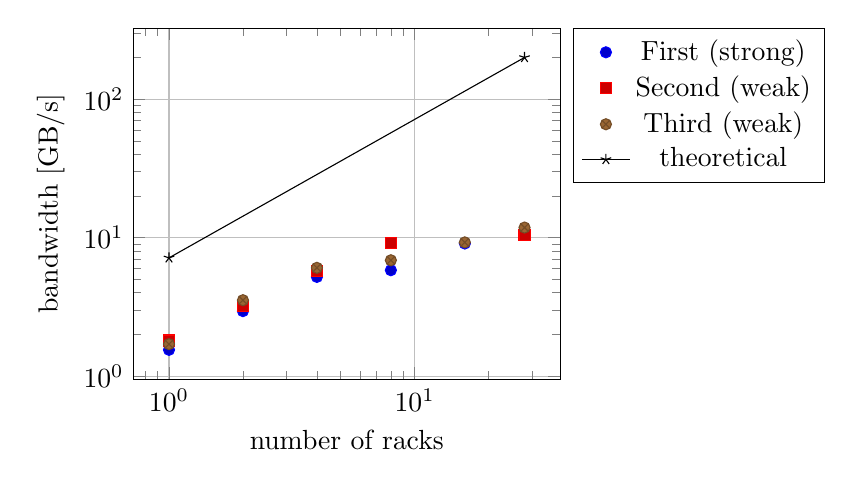
\begin{tikzpicture}
\begin{loglogaxis}[
    %title=Measured bandwidth,
    xlabel={number of racks},
    ylabel={bandwidth [GB/s]},
    grid=major,
    legend entries={First (strong),Second (weak),Third (weak),theoretical},
    legend pos = outer north east
]
\addplot+[only marks] plot coordinates {
	(1,1.5467661232)
	(2,2.9454691765) 
  	(4,5.2017538625)
  	(8,5.8155415474)
  	(16,9.0672199939)
  	(28,11.2385628539)};
\addplot+[only marks] plot coordinates {
	(1,1.806100989)
	(2,3.1885595039) 
  	(4,5.720142807)
  	(8,9.1409379542)
  	(28,10.3862295069)};
\addplot+[only marks] plot coordinates {
	(1,1.7024458792)
	(2,3.532729664) 
  	(4,6.0497625907)
  	(8,6.8614197141)
  	(16,9.239307873)
  	(28,11.8209114989)};
\addplot plot coordinates {
	(1,7.14) 
	(28,200)};
\end{loglogaxis}
\end{tikzpicture}
\end{document}